\documentclass{beamer}
\usetheme[%
progressbar=frametitle,
subsectionpage=none
]{metropolis}

\usepackage{fontspec}
\setsansfont{Source Sans Pro}
\setmonofont{Source Code Pro}

\usepackage{polyglossia}
\setmainlanguage{german}
\setotherlanguage{english}

\usepackage[smaller]{acronym}
\usepackage{biblatex}
\usepackage[german=guillemets]{csquotes}
\usepackage{fontawesome}
\usepackage{framed}
\usepackage{hyperref}
\usepackage{listings}
%\usepackage{microtype}
\usepackage{xcolor}
\usepackage{xspace}

\title{\ac{SANE}}
\subtitle{Ein neuer Versuch}
\author{David Sukiennik}
%\date{\today}
\institute[FG IKS]{Fachgebiet Integrierte Kommunikationssysteme}

\setbeamercovered{dynamic}

\hypersetup{%
	unicode=true
}

\bibliography{pres}

\newcommand{\et}{\textit{\&}\xspace}
\newcommand{\zB}{z.\,B.\xspace}
\newcommand{\basedgfx}[1]{\raisebox{-.3\baselineskip}{\includegraphics[height=\baselineskip]{#1}}}
\newcommand{\inlinegfx}[1]{\raisebox{-.2\baselineskip}{\includegraphics[height=.7\baselineskip]{#1}}}

\lstset{%
	frame=l,
	basicstyle=\footnotesize,
	commentstyle=\color{gray}\sffamily,
	identifierstyle=\color{black},
	keywordstyle=\color{mLightBrown},
	numberstyle=\color{gray},
	stringstyle=\color{red}\ttfamily
}

\lstdefinelanguage{HTML5}{%
	language=html,
	morecomment=[s]{<!-}{-->},
	tag=[s],
	otherkeywords={%
		% Standard tags
		<!DOCTYPE,
		html, /html, head, /head, title, /title, style, link, meta,
		% body
		body, /body,
		% Divs
		div,
		% scripts
		script,
		% More tags...
		canvas, svg, rect, animateTransform, video, source, iframe, video, image
	},
	ndkeywords={%
		% General
		=,
		% HTML attributes
		charset=, src=, id=, width=, height=, style=, type=, rel=, href=,
		% SVG attributes
		fill=, attributeName=, begin=, dur=, from=, to=, poster=, controls=, x=, y=, repeatCount=, xlink:href=,
		% CSS properties
		margin:, padding:, background-image:, border:, top:, left:, position:, width:, height:,
		% CSS3 properties
		transform:, -moz-transform:, -webkit-transform:,
		animation:, -webkit-animation:,
		transition:,  transition-duration:, transition-property:, transition-timing-function:,
	}
}

\lstdefinelanguage{JavaScript}{%
	keywords={typeof, new, true, false, catch, function, return, null, catch, switch, var, if, in, while, do, else, case, break, const, let, class},
	ndkeywords={class, export, boolean, throw, implements, import, this, document, body},
	ndkeywordstyle=\color{darkgray}\bfseries,
	identifierstyle=\color{black},
	sensitive=false,
	comment=[l]{//},
	morecomment=[s]{/*}{*/},
	commentstyle=\color{purple}\ttfamily,
	morestring=[b]',
	morestring=[b]" % chktex 18
}

\lstdefinelanguage{TypeScript}{%
	language=JavaScript,
	morekeywords={const, let, class, constructor, public, private, protected, enum, interface},
	sensitive=false,
}



\begin{document}
\maketitle

\begin{frame}{Outline}
	\setcounter{tocdepth}{1}
	\tableofcontents
\end{frame}

\section{Bisheriger Stand}
\begin{frame}{Bisheriger Stand}
	\begin{columns}[onlytextwidth]
		\column{0.6\textwidth}
		\begin{itemize}
			\item einzelne Java-Applets für \zB\ Karnaugh-Plan, Venn-Diagramm etc.
			\item zusammengeführt in der \ac{SANE}-Workstation
		\end{itemize}

		\column{0.4\textwidth}

		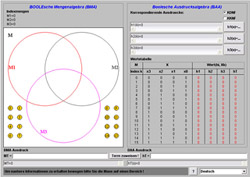
\includegraphics[width=0.8\textwidth]{gfx/bmma_klein.jpg}

		\medskip

		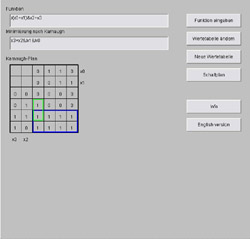
\includegraphics[width=0.8\textwidth]{gfx/karnaugh_klein.jpg}
	\end{columns}
\end{frame}

\subsection{Probleme}
\begin{frame}{Probleme}
	\begin{itemize}
		\item Java wird nicht mehr von Browsern unterstützt
			\begin{itemize}
				\item Firefox seit v53 (2017)
				\item Chrome seit v45 (2015)
			\end{itemize}
		\item Code entstand über viele Jahre in studentischen Arbeiten
			\begin{itemize}
				\item Code ist veraltet, nicht einheitlich und ergo nicht wartbar
			\end{itemize}
		\item Aussehen, Performance, Plattform nicht auf modernem Stand
	\end{itemize}
\end{frame}

\section{Entwurf \& Design}
\metroset{subsectionpage=progressbar}
\subsection{Anforderungen}
\begin{frame}{Anforderungen}
	\begin{itemize}
		\item Plattformunabhängigkeit
		\item Unterstützung auch mobiler Plattformen
		\item einheitliche, moderne Code-Basis
			\begin{itemize}
				\item wartbar
			\end{itemize}
	\end{itemize}
\end{frame}

\subsection{Lösungsvorschlag}
\begin{frame}{Lösungsvorschlag}
	\begin{itemize}
		\item Nutzung des Browsers als Plattform statt Plugins
			\begin{itemize}
				\item »plattformunabhängigste Plattform«: alle Betriebssysteme, vom Desktop bis zum Smartphone
				\item \ac{JS}, \ac{HTML}, \ac{DOM}
			\end{itemize}
		\item einheitliche Code-Struktur und -Stil
		\item einheitlicher Datenflusses
		\item responsives, modernes Layout
	\end{itemize}
\end{frame}

\subsection{Kerntechnologien}
\begin{frame}{Kerntechnologien}
	\begin{itemize}
		\item \ac{TS}:~\basedgfx{gfx/TypeScript-logo}
		\item Polymer:~\basedgfx{gfx/p-logo}
		\item Automatisierung (\basedgfx{gfx/npm}/\basedgfx{gfx/yarn-kitten-full}, \basedgfx{gfx/gulp} gulp), Linter (TSLint), …
	\end{itemize}
\end{frame}

\subsection{TypeScript}
\begin{frame}{TypeScript}
	\begin{itemize}
		\item typisiertes \acl{JS}: erleichtert Programmierung und Debugging
			\begin{itemize}
				\item statische Typprüfung zur Übersetzungszeit → \zB\ korrekter Funktionsaufruf?
				\item Refactoring wird erleichtert
				\item Angabe der Interfaces erleichtert Verständnis der erwarteten Schnittstellen
			\end{itemize}
		\item Transpilation in \acl{JS} erlaubt Nutzung auf Browsern
		\item Nutzung moderner \ac{JS}-Technologien (teilweise bis \ac{ES} 7: Klassen, einfacheres Scoping, …) während der Entwicklung
			\begin{itemize}
				\item Transpilation in alten Code erlaubt Nutzung auch in Browsern ohne Unterstützung neuer Features
			\end{itemize}
		\item von Microsoft
	\end{itemize}
\end{frame}

\subsection{Polymer}
\begin{frame}{Polymer~\basedgfx{gfx/p-logo}}
	\begin{itemize}
		\item Framework, um Web Components und weitere moderne Browsertechnologien einfacher zu nutzen
		\item Erstellung eigener, wiederverwendbarer und gekapselter \acs{HTML}-Elemente
		\item grundlegende Elemente bereits erstellt mit modernem Anspruch auf Responsivität, Wiederverwendbarkeit und modernem Aussehen
		\item von Google
	\end{itemize}
\end{frame}

\subsubsection{Komposition}
\begin{frame}{Komposition}
	\begin{itemize}
		\item Custom Elements bestehen aus mehreren Elementen
		\item Custom Elements können auch aus weiteren Custom Elements bestehen
		\item komplexe Elemente: Komposition aus Elementen
		\item Vorteile:
			\begin{itemize}
				\item Kapselung
				\item Abstraktion
				\item Wiederverwendbarkeit
			\end{itemize}
	\end{itemize}
\end{frame}

\subsubsection{Datenfluss}
\begin{frame}{Datenfluss}
	\begin{itemize}
		\item Unidirektionaler Datenfluss
		\item Data Binding von \enquote{oben nach unten}, also Eltern- zu Kinderelementen
			\begin{itemize}
				\item One-Way Data Binding erlaubt lesenden, aber keinen schreibenden Zugriff
			\end{itemize}
		\item Kinderelemente kommunizieren per Events Änderungswünsche
			\begin{itemize}
				\item Events \enquote{bubblen} nach oben
			\end{itemize}
		\item mehrere Elemente (≙= Module) möchten Änderungen vornehmen
			\begin{itemize}
				\item Zentralisierung und Vereinheitlichung des Datenflusses erleichtert Verständnis und Debugging
				\item Einheitliche Event-Namen, die alle Module verwenden können und sollen
			\end{itemize}
		\item \texttt{<sane-data>} verwaltet Daten
	\end{itemize}
\end{frame}

\subsection{Toolchain}
\subsubsection{Build}
\begin{frame}{Build}
	Build wird als npm-Script ausgeführt
	\begin{enumerate}
		\item \emph{Linting} erzwingt einheitlichen Style und vermeidet klassische Fehler
			\pause
		\item \emph{Transpilation von \acl*{TS} in \acl*{JS}} prüft statisch auf Korrektheit der Interfaces (Typisierung) und wandelt den Code in JavaScript um
			\pause
		\item \emph{Polymer Build} minifyt \acs{HTML}, \acs{CSS} und \ac{JS} und erstellt Service Worker
	\end{enumerate}
			\pause
	\begin{description}
		\item[Resultat:] eine App; entwickelt mit moderner, einheitlicher Technologie; lauffähig auf allen modernen Browsern
	\end{description}
\end{frame}

\begin{frame}{Build}
	\begin{figure}
		\centering
		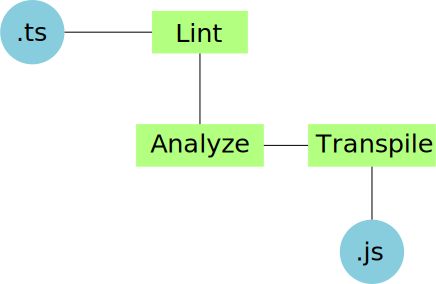
\includegraphics[width=\textwidth]{gfx/TypeScript2JavaScript}
		\caption{\inlinegfx{gfx/TypeScript-logo} zu JavaScript}
		\label{fig:TS2JS}
	\end{figure}
\end{frame}

\begin{frame}{Build}
	\begin{figure}
		\centering
		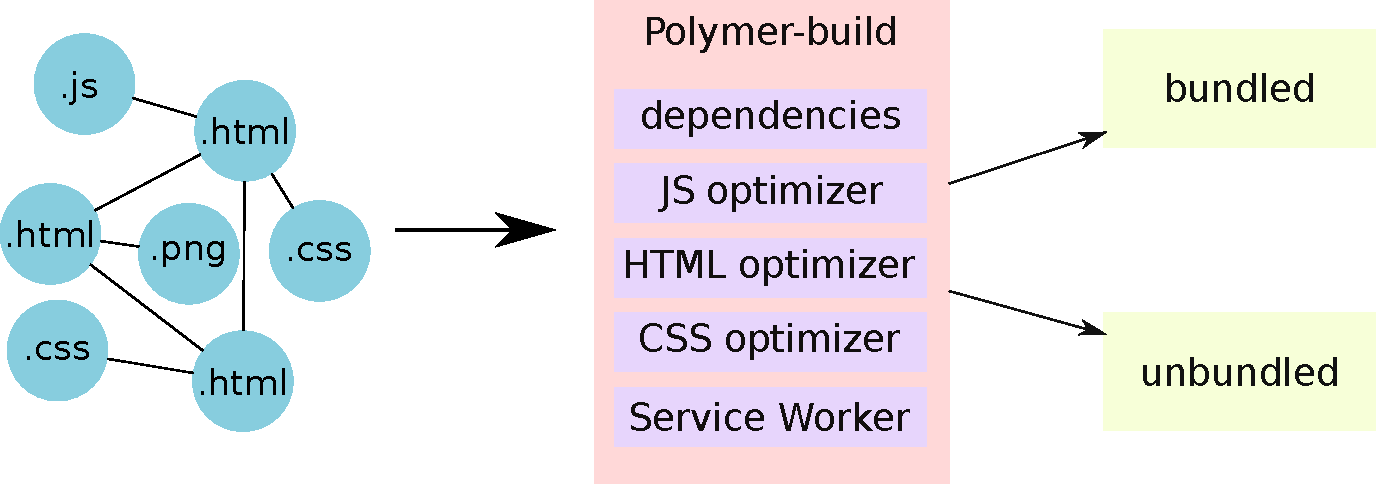
\includegraphics[width=\textwidth]{gfx/Polymer-build}
		\caption{Polymer-build}
		\label{fig:polymer-build}
	\end{figure}
\end{frame}

\section{Beispiele}
\subsection{TypeScript}
\begin{frame}[fragile]{Transpiliertes JavaScript: \texttt{enum}}
	\begin{minipage}{.4\textwidth}
		\lstinputlisting[language=TypeScript, numbers=left, breaklines=true, basicstyle=\scriptsize, linerange={1-6}, caption={TypeScript: \texttt{enum}}]{src/example1.ts}
	\end{minipage}
	\hfill
	\begin{minipage}{.5\textwidth}
		\lstinputlisting[language=Javascript, numbers=left, breaklines=true, basicstyle=\tiny, linerange={1-7}, caption={JavaScript: IIFE}]{src/example1.js}
	\end{minipage}
\end{frame}

\begin{frame}[fragile]{Transpiliertes JavaScript: Interfaces}
	\lstinputlisting[language=TypeScript, numbers=left, breaklines=true, basicstyle=\scriptsize, linerange={8-11}, caption={TypeScript: Interfaces}]{src/example1.ts}
\end{frame}

%\begin{frame}[fragile]{Transpiliertes JavaScript: \texttt{class}}
%	\begin{minipage}{.45\textwidth}
%		\lstinputlisting[language=TypeScript, numbers=left, breaklines=true, basicstyle=\tiny, linerange={13-18}, caption={TypeScript: \texttt{class}}]{src/example1.ts}
%	\end{minipage}
%	\hfill
%	\begin{minipage}{.45\textwidth}
%		\lstinputlisting[language=Javascript, numbers=left, breaklines=true, basicstyle=\tiny, linerange={8-17}, caption={JavaScript: IIFE}]{src/example1.js}
%	\end{minipage}
%\end{frame}

\begin{frame}[fragile]{Transpiliertes JavaScript: \texttt{class}}
	\lstinputlisting[language=TypeScript, numbers=left, breaklines=true, basicstyle=\tiny, linerange={13-18}, caption={TypeScript: \texttt{class}}]{src/example1.ts}
	\hfill
	\lstinputlisting[language=Javascript, numbers=left, breaklines=true, basicstyle=\tiny, linerange={8-17}, caption={JavaScript: IIFE}]{src/example1.js}
\end{frame}


\begin{frame}[fragile]{Transpiliertes JavaScript}
%	\begin{minipage}{.45\textwidth}
		\lstinputlisting[language=TypeScript, numbers=left, breaklines=true, basicstyle=\tiny, linerange={20-21}, caption={TypeScript}]{src/example1.ts}
%	\end{minipage}
	\hfill
%	\begin{minipage}{.45\textwidth}
		\lstinputlisting[language=Javascript, numbers=left, breaklines=true, basicstyle=\tiny, linerange={19-20}, caption={JavaScript}]{src/example1.js}
%	\end{minipage}
\end{frame}

\begin{frame}[fragile]{TypeScript}
	\lstinputlisting[language=TypeScript, numbers=left, breaklines=true, basicstyle=\tiny]{src/example1.ts}
\end{frame}

\begin{frame}[fragile]{Transpiliertes JavaScript}
	\lstinputlisting[language=Javascript, numbers=left, breaklines=true, basicstyle=\tiny]{src/example1.js}
\end{frame}


\subsection{Web Components \& Polymer}
\begin{frame}{Beispiel-Element}
	Beispielelement \texttt{<paper-slider>}:

	\url{https://www.webcomponents.org/element/PolymerElements/paper-slider/demo/demo/index.html}
\end{frame}

\subsection{\texttt{index.html}}
\begin{frame}[fragile]{\texttt{index.html}}
	\begin{lstlisting}[%
		language=HTML5,
		texcl=true,
		tagstyle=\color{blue},
		alsodigit={-},
		emph={sane-app},
		emphstyle={\color{mLightGreen}\bfseries}
		]
<html>
  <head>
    <!-- … -->
    <title>Schaltsysteme Arbeitsblätter im Netz</title>
    <!-- … -->
  </head>
  <body>
  <sane-app></sane-app> <!-- ⚡eigenes HTML-Element⚡ -->
  </body>
</html>
	\end{lstlisting}
	Das war's! \faSmileO
\end{frame}

\subsubsection{Data Binding}
\begin{frame}[fragile]{Data-Binding}
	\begin{lstlisting}[%
		language=HTML5,
		numbers=left,
		tagstyle=\color{blue},
		breaklines=true,
		alsodigit={-[]},
		alsoletter={[]},
		emph={\[\[,\]\]},
		emphstyle={\color{mLightGreen}\bfseries}
	]
<iron-pages selected="[[page]]" attr-for-selected="name" fallback-selection="view404" role="main">
  <sane-view1 name="view1" language="[[language]]" data="[[sanedata]]"></sane-view1>
  <sane-view2 name="view2" language="[[language]]" data="[[sanedata]]"></sane-view2>
  <sane-view3 name="view3" language="[[language]]" data="[[sanedata]]"></sane-view3>
  <sane-view404 name="view404"></sane-view404>
</iron-pages>
	\end{lstlisting}
\end{frame}

\subsection{Aktueller Stand von \ac{SANE}}
\begin{frame}{Demo: Beispielfunktionalitäten}
	\begin{itemize}
		\item Truth Table
		\item Language Switch
		\item On-Demand Loading
		\item Responsives Design
		\item Quasi-Native app
	\end{itemize}
\end{frame}


\metroset{subsectionpage=none}
\section{Ausblick}
\subsection{Geplante Module}
\begin{frame}{Geplante Module}
	\begin{itemize}
		\item Wahrheitstabelle
		\item Mengendiagramm
		\item Karnaugh-Diagramm
		\item  $g$-Parameter-Bestimmung
		\item …
	\end{itemize}
	Unter Nutzung der vorhandenen Schnittstellen lassen sich beliebige Module hinzufügen.
\end{frame}

\subsection{Splitscreen}
\begin{frame}{Splitscreen}
	\begin{figure}[]
		\centering
		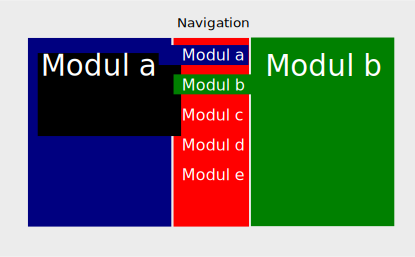
\includegraphics[width=\textwidth]{gfx/splitscreen}
		\caption{Abstrahiertes Konzept des Splitscreens}
		\label{fig:splitscreen}
		\end{figure}
\end{frame}

\begin{frame}[standout]
	Dankeschön!
\end{frame}

\appendix

\begin{frame}{Abkürzungsverzeichnis}
	\begin{acronym}
		\acro{CSS}{Cascading Style Sheet}
		\acro{DOM}{Document Object Model}
		\acro{ES}{ECMAScript}
		\acro{HTML}{HyperText Markup Language}
		\acro{JS}{JavaScript}
		\acro{SANE}{Schaltsysteme Arbeitsblätter im Netz}
		\acro{TS}{TypeScript}
	\end{acronym}
\end{frame}

\begin{frame}[allowframebreaks]{Literaturverzeichnis}
	\nocite{*}
	\printbibliography
\end{frame}

\end{document}
